
%% Uncomment one of these:
%% the 1st when using pdflatex, which directly typesets your document in
%% pdf (use jpg or pdf figures), or
%% the 2nd when producing a ps file (use eps figures, don't use ps figures!).
\documentclass[english,12pt,a4paper,pdftex,elec,utf8]{aaltothesis}
%\documentclass[english,12pt,a4paper,dvips]{aaltothesis}

%% To the \documentclass above
%% specify your school: arts, biz, chem, elec, eng, sci
%% specify the character encoding scheme used by your editor: utf8, latin1

%% Use one of these if you write in Finnish (see the Finnish template):
%%
%\documentclass[finnish,12pt,a4paper,pdftex,elec,utf8]{aaltothesis}
%\documentclass[finnish,12pt,a4paper,dvips]{aaltothesis}

\usepackage{graphicx}

%% Use this if you write hard core mathematics, these are usually needed
\usepackage{amsfonts,amssymb,amsbsy}

%% Use the macros in this package to change how the hyperref package below 
%% typesets its hypertext -- hyperlink colour, font, etc. See the package
%% documentation. It also defines the \url macro, so use the package when 
%% not using the hyperref package.
%%
%\usepackage{url}

%% Use this if you want to get links and nice output. Works well with pdflatex.
\usepackage{hyperref}
\hypersetup{pdfpagemode=UseNone, pdfstartview=FitH,
  colorlinks=true,urlcolor=red,linkcolor=blue,citecolor=black,
  pdftitle={Default Title, Modify},pdfauthor={Your Name},
  pdfkeywords={Modify keywords}}


%% All that is printed on paper starts here
\begin{document}

%% Change the school field to specify your school if the automatically 
%% set name is wrong
% \university{aalto-yliopisto}
% \university{aalto University}
% \school{Sähkötekniikan korkeakoulu}
% \school{School of Electrical Engineering}

%% Only for B.Sc. thesis: Choose your degree programme. 
%\degreeprogram{Electronics and electrical engineering}
%%

%% ONLY FOR M.Sc. AND LICENTIATE THESIS: Specify your department,
%% professorship and professorship code. 
%%
\department{Department of Radio Science and Technology}
%\professorship{Circuit theory}
%%

%% Valitse yksi näistä kolmesta
%%
%% Choose one of these:
%\univdegree{BSc}
%\univdegree{MSc}
%\univdegree{Lic}

%% Your own name (should be self explanatory...)
\author{Jiri Burant}

%% Your thesis title comes here and again before a possible abstract in
%% Finnish or Swedish . If the title is very long and latex does an
%% unsatisfactory job of breaking the lines, you will have to force a
%% linebreak with the \\ control character. 
%% Do not hyphenate titles.
%% 
\thesistitle{Virtual image generator for asteroid mission navigation}

\place{Espoo}

%% For B.Sc. thesis use the date when you present your thesis. 
%% 
%% Kandidaatintyön päivämäärä on sen esityspäivämäärä! 
%%\date{16.1.2015}

%% B.Sc. or M.Sc. thesis supervisor 
%% Note the "\" after the comma. This forces the following space to be 
%% a normal interword space, not the space that starts a new sentence. 
%% This is done because the fullstop isn't the end of the sentence that
%% should be followed by a slightly longer space but is to be followed
%% by a regular space.
%%
\supervisor{Prof.\ Esa Kallio} %{Prof.\ Pirjo Professori}

%% B.Sc. or M.Sc. thesis advisors(s). You can give upto two advisors in
%% this template. Check with your supervisor how many official advisors
%% you can have.
%%
%\advisor{Prof.\ Pirjo Professori}
%%\advisor{D.Sc.\ (Tech.) Olli Ohjaaja}
%\advisor{M.Sc.\ Polli Pohjaaja}

%% Aalto logo: syntax:
%% \uselogo{aaltoRed|aaltoBlue|aaltoYellow|aaltoGray|aaltoGrayScale}{?|!|''}
%%
%% Logo language is set to be the same as the document language.
%% Logon kieli on sama kuin dokumentin kieli
%%
\uselogo{aaltoRed}{''}

%% Create the coverpage
%%
\makecoverpage


%% Note that when writting your master's thesis in English, place
%% the English abstract first followed by the possible Finnish abstract

%% English abstract.
%% All the information required in the abstract (your name, thesis title, etc.)
%% is used as specified above.
%% Specify keywords
%%
%% Kaikki tiivistelmässä tarvittava tieto (nimesi, työnnimi, jne.) käytetään
%% niin kuin se on yllä määritelty.
%% Avainsanat
%%
\keywords{Image generator, space technology project, openGL, java}
%% Abstract text
\begin{abstractpage}[english]
This project deals with testing of possible setups of a camera mounted on spacecraft. The idea is to simulate simplified movement of this spacecraft above the surface 
and capture images along the way. Based on those images, it can be decided which camera is best suitable for the given mission and at which angle it should be facing. 
The generated images can also be used in the next stage to test image analysis tools or image reconstruction software. 

To do so, a simple application has been developped in java programming language, simulating the movement of the spacecraft and generating the pictures. It consists of a big canvas with 
2D image, above which the spacecraft moves and simple GUI, allowing the user to change basic parameters such as the altitude of the spacecraft, the angle of the mounted camera and do on.

The basic application has been developped and tested, giving satisfying results, but there is a lot of room for future extensions, some of them being described in this report.
\end{abstractpage}

%% Force a new page so that the possible English abstract starts on a new page
%%
%% Pakotetaan uusi sivu varmuuden vuoksi, jotta 
%% mahdollinen suomenkielinen ja englanninkielinen tiivistelmä
%% eivät tule vahingossakaan samalle sivulle
\newpage
%


%% Preface
%%
%% Esipuhe 
\mysection{Preface}
%\mysection{Esipuhe}
I want to thank Professor Esa Kallio for the opportunity to work on this project and for his guidance and optimism.\\

\vspace{5cm}
Helsinky, 6.11.2016

\vspace{5mm}
{\hfill Jiri Burant \hspace{1cm}}

%% Force new page after preface
%%
%% Pakotetaan varmuuden vuoksi esipuheen jälkeinen osa
%% alkamaan uudelta sivulta
\newpage


%% Table of contents. 
\thesistableofcontents


%% Symbols and abbreviations
%%\mysection{Symbols and abbreviations}
%%
%%\subsection*{Symbols}
%%
%%\begin{tabular}{ll}
%%$\mathbf{B}$  & magnetic flux density  \\
%%$c$              & speed of light in vacuum $\approx 3\times10^8$ [m/s]\\
%%$\omega_{\mathrm{D}}$    & Debye frequency \\
%%$\omega_{\mathrm{latt}}$ & average phonon frequency of lattice \\
%%$\uparrow$       & electron spin direction up\\
%%$\downarrow$     & electron spin direction down
%%\end{tabular}
%%
%%\subsection*{Operators}
%%
%%\begin{tabular}{ll}
%%$\nabla \times \mathbf{A}$              & curl of vectorin $\mathbf{A}$\\
%%$\displaystyle\frac{\mbox{d}}{\mbox{d} t}$ & derivative with respect to 
%%variable $t$\\[3mm]
%%$\displaystyle\frac{\partial}{\partial t}$  & partial derivative with respect 
%%to variable $t$ \\[3mm]
%%$\sum_i $                       & sum over index $i$\\
%%$\mathbf{A} \cdot \mathbf{B}$    & dot product of vectors $\mathbf{A}$ and 
%%$\mathbf{B}$
%%\end{tabular}
%%
%%\subsection*{Abbreviations}
%%
%%\begin{tabular}{ll}
%%AC         & alternating current \\
%%APLAC      & an object-oriented analog circuit simulator and design tool \\
%%           & (originally Analysis Program for Linear Active Circuits) \\
%%BCS        & Bardeen-Cooper-Schrieffer \\ %% dash between the names
%%DC         & direct current \\
%%TEM        & transverse eletromagnetic
%%\end{tabular}


%% Tweaks the page numbering to meet the requirement of the thesis format:
%% Begin the pagenumbering in Arabian numerals (and leave the first page
%% of the text body empty, see \thispagestyle{empty} below).
%% Additionally, force the actual text to begin on a new page with the 
%% \clearpage command.
%% \clearpage is similar to \newpage, but it also flushes the floats (figures
%% and tables).
%% There is no need to change these
%%
\cleardoublepage
\storeinipagenumber
\pagenumbering{arabic}
\setcounter{page}{1}


%% Text body begins. Note that since the text body
%% is mostly in Finnish the majority of comments are
%% also in Finnish after this point. There is no point in explaining
%% Finnish-language specific thesis conventions in English. Someday 
%% this text will possibly be translated to English.
%%
\section{Introduction}

The project of the virtual image generator has been developped as a helper software tool for the ASPECT project \cite{ASPECT}, which is part of the ESA's Asteroid Impact Misstion (AIM) \cite{AIM}.

The goal of the AIM is to demonstrate new technologies, mainly in the telecommunications domain. The AIM mission will consist of the main spacecraft carrying the Mascot-2 asteroid lander,  as well as two or more CubeSats. The mission should launch in in October 2020, then travel to the Didymos asteriod pair. The spacecraft would perform high-resolution visual, thermal and radar mapping of the moon and build detailed maps of its surface and interior structure. 

The ASPECT project focuses on developping a single three-unit CubeSat equipped with a visible/near-infrared spectrometer to assess the asteroid composition and effects of space weathering and metamorphic shock, as well as post-impact plume observations. 

The Cubesat will be deployed from a 10 km height from the target's surface and orbit it at around 1 to 3 km from the surface. From this distance it will measure the reflectance which will give an understanding of the composition of Didymoon and may provide answers to how this is influenced by space weathering and shock effect.

The navigation of the ASPECT CubeSat is a problematic task, and one of the things that could help it are the camera images. By using appropriate camera and appropriate software, position and speed could be estimated by analyzing the captured images. In order to determine a feasible camera setup and to test the analysis software, before it is deployed to the spacecraft, The Virtual Image Generator, VGI tool has been developped.

It simulates the movement of the spacecraft above surface along specified trajectory (assumed as line), capturing images below. Those images are saved as screenshots, and can later be used for testing image reconstruction, mapping software or speed and position estimation software.

The outcome of this work is a basic software application, ready for future extensions. Some of possible future improvements or applications are discussed in section 4. of this report.

\clearpage

\section{Software design}
\subsection*{Basic information}
The application has been developped in java programming language, using JDK 1.8\cite{java} and NetBeansIDE\cite{NetBeans}. Apart from that, openGL in form of lwjgl \cite{lwjgl} library has been used, details can be found on official pages or in Appendix A.

\subsection*{Architecture description}
The application project itself consists of two packages. 
Package called \textit{utils} consists of parts of the source code from the joml java library. It contains classes and methods for manipulating vectors and matrices, which is useful when rendering the openGL objects. 
Package \textit{cameraproject} comprises all the application logic. It contains classes concerning the openGL tasks, as texture loading and scene rendering, it also contains the GUI setup and operation logic.

The code itself is thoroughly documented and self-explanatory. Nevertheless, a brief description of the most important classes follows.

The main class is called \textit{CameraProject.java} In this class, the basic GUI initialization is carried out as well as the openGL initialization. Moreover, the main rendering loop is also located there.

For each of the rendered objects, that means the target location, the surface plane and the spacecraft, a dedicated class containing the parameters for the given object, has been created. Those classes are named: \textit{Target.java}, \textit{Land.java} and \textit{Carrier.java}, respectivelly. These three classes have a common parent named \textit{SceneObject.java}, which contains the common parameters, that each scene object must have, as Texture \textit{Texture.java} and Model \textit{Model.java}. Class \textit{Texture.java} contains the loaded texture for the given object and the class \textit{Model.java} contains parameters and methods for rendering of the scene objects.

Class named \textit{Shader.java} is purely openGL based, and creates the shaders for rendering. The shaders specify, how should each pixel be rendered (color, texture, attenuation and so on.)

Class \textit{Camera.java} contains the parameter of the camera, such as field of view, angles of the camera and so on. From those parameters, a transformation matrix is computed, which serves for rendering of the "observed" objects.

The remaining classes \textit{TextFieldListener.java}, \textit{FloatWrapper.java} and \textit{InputData.java} are helper classes, which facilitate the transport of data from the GUI text fields into the program.

\subsection*{Graphical User Interface}

The GUI has been developped using the java's native Swing library. The GUI is simple and comprises of several labels and text fields for entering the input data and two buttons, one for starting the simulation, one for loading the texture. The layout has been chosen as box layout, because it is straightforward and easy to modify.

In the fig.\ref{GUIExample}, there is an example of how the running apllication looks like. On the left side, there is a surface (land) covered with texture of an island. Over it, a blue and a smaller red rectangles are drawn. They symbolize the spacecraft (carrier) and the target. On the right side, the GUI panel is shown. First field is number of images to be taken during the flight. The second field specifies the output image type, for the time being there are just two options, \textit{.jpg} and \textit{.png.}Underneath, there is the initial position of the spacecraft, the three coordinates specify the x,y,z position in the respective coordinate system. The trajectory's end position specifies the target location. Last fields are camera parameters, namely two angles of the camera measured as deviation from the x, respectively y axis, specified in radians, and the field of view of the camera, specified in degrees. Finally, there are buttons for starting the simulation and for loading of the surface texture.

\begin{figure}[htb]
\centering 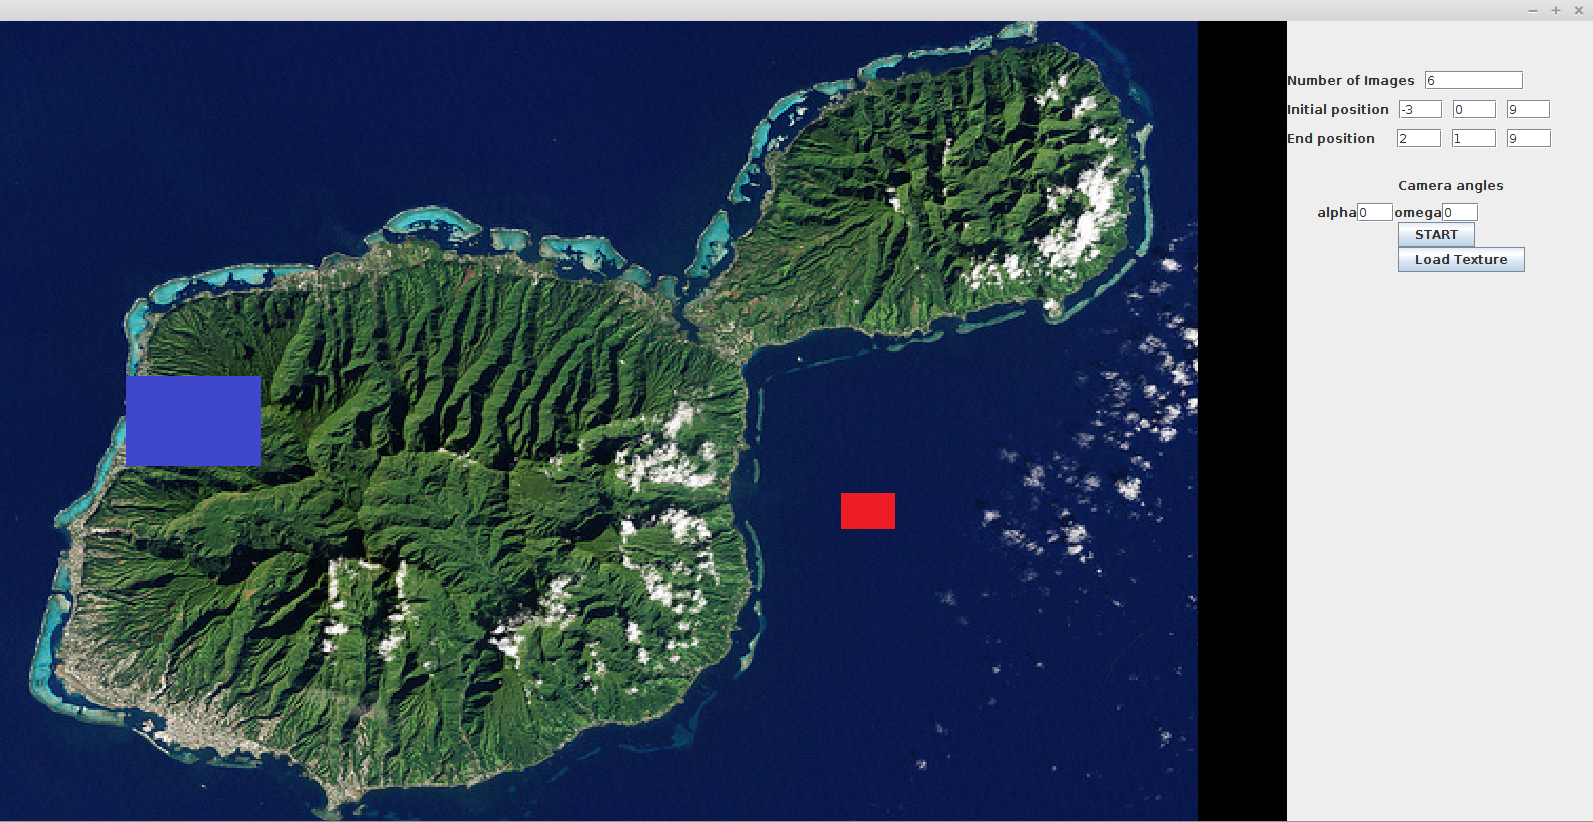
\includegraphics[height=7cm]{GUIExample.png}
\caption{Example run of the application\label{GUIExample}}
\end{figure}

The coordinate system of the rendered left part of the window is classical 3D Cartesian system, which spans from -4.5 to 4.5 for the x and y coordinates. For the z coordinates, it spans from 0 to 10, while 10 being the coordinate of the surface plane. Therefore the z coordinate is somewhat reversed altitude, as 0 is at the overview, top camera location and 10 is on the surface. 

Once the simulation starts, the camera switches to view of the camera mounted on the spacecraft, with the specified parameters. The images captured by the spacecraft are rendered and consequently saved into a file. A few examples of such images are presented in the section 3.

\clearpage

\section{Results}

The system has been tested on a laptop with following specifications. Operating system: LinuxMint 17, Processor: Intel Pentium B970 2.3GHz, RAM: 4GB, integrated graphics card.

The application was tested for several different setups of camera parameters, different positions of the spacecraft and number of steps. 

Following figures depict two example cases, their setup and the resulting screenshots, for both tests 4 steps were chosen.

In the first example case the spacecraft flew from coordinates [-3,-3,9] to coordinates [3,3,9]

In the second example case the spacecraft flew from coordinates [-3,3,7] to coordinates [2,-1,9], because it started on z coordinate 7, it was outside of the camera scope, therefore there it is not visible in the setup figure.
Also, the omega angle has been chosen as -0.01rad, therefore the image is slightly tilted.

The results of those tests were quite convincing, and they suggest, that the image generation works correctly.

\begin{figure}[htb]
\centering 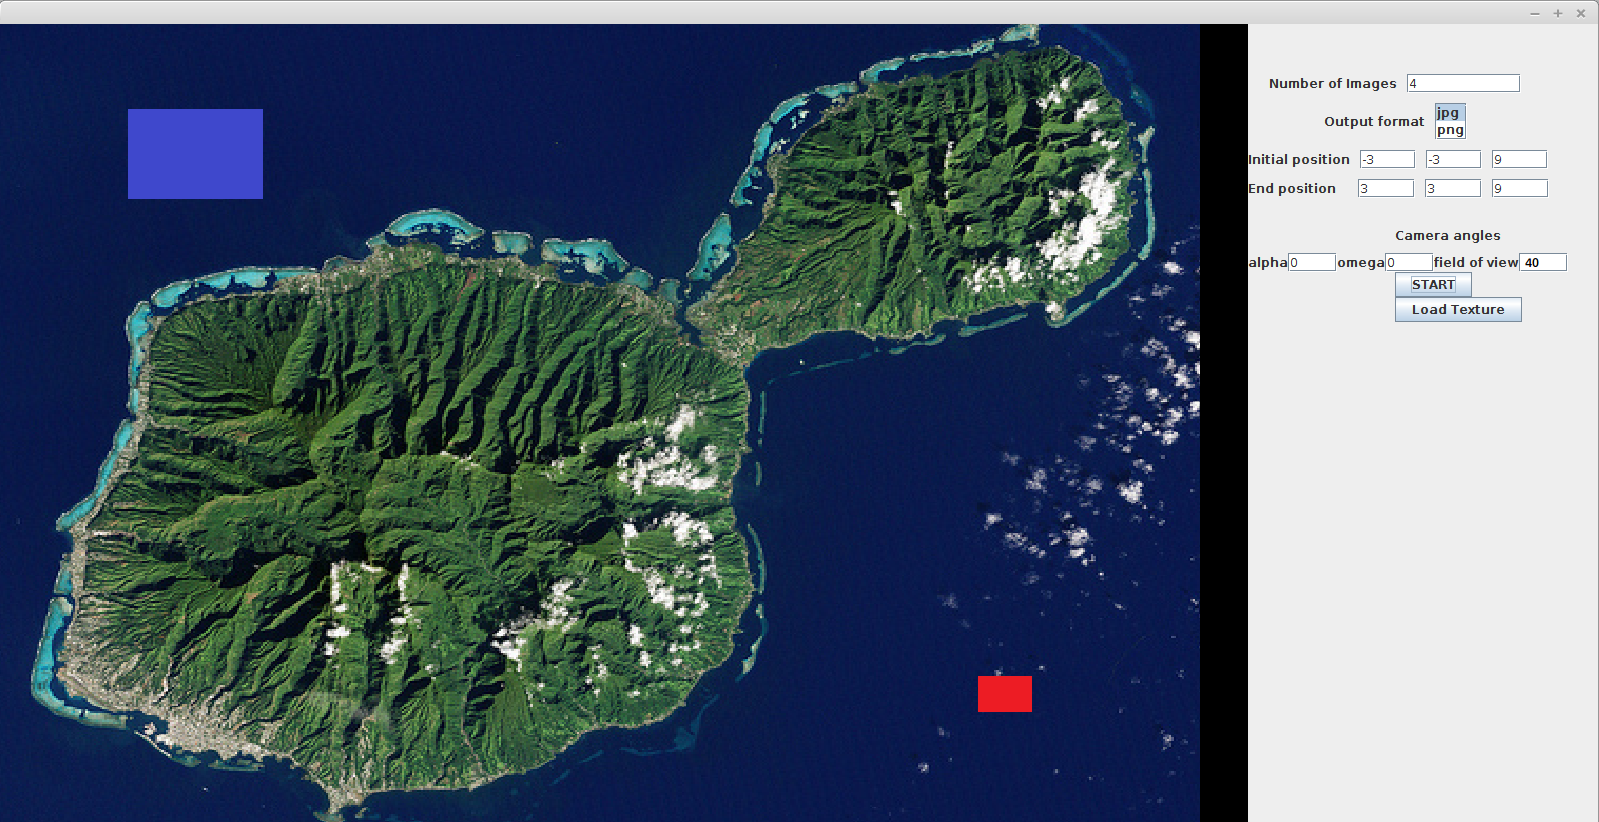
\includegraphics[height=7cm]{screenTest1.png}
\caption{The setup of the first test\label{screenTest1}}
\end{figure}

\begin{figure}[htb]
\centering 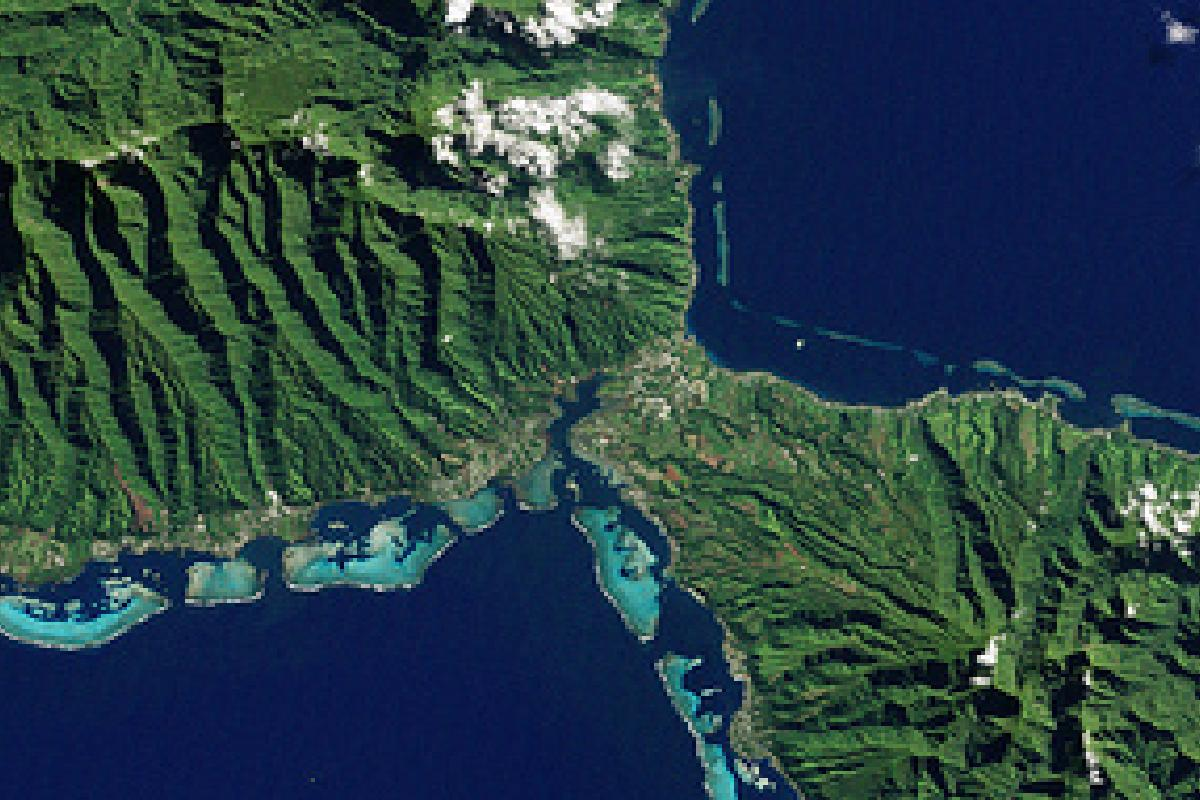
\includegraphics[height=5cm]{screenshot00.jpg}
\caption{First step of the first test\label{screenshot0Test1}}
\end{figure}

\begin{figure}[htb]
\centering 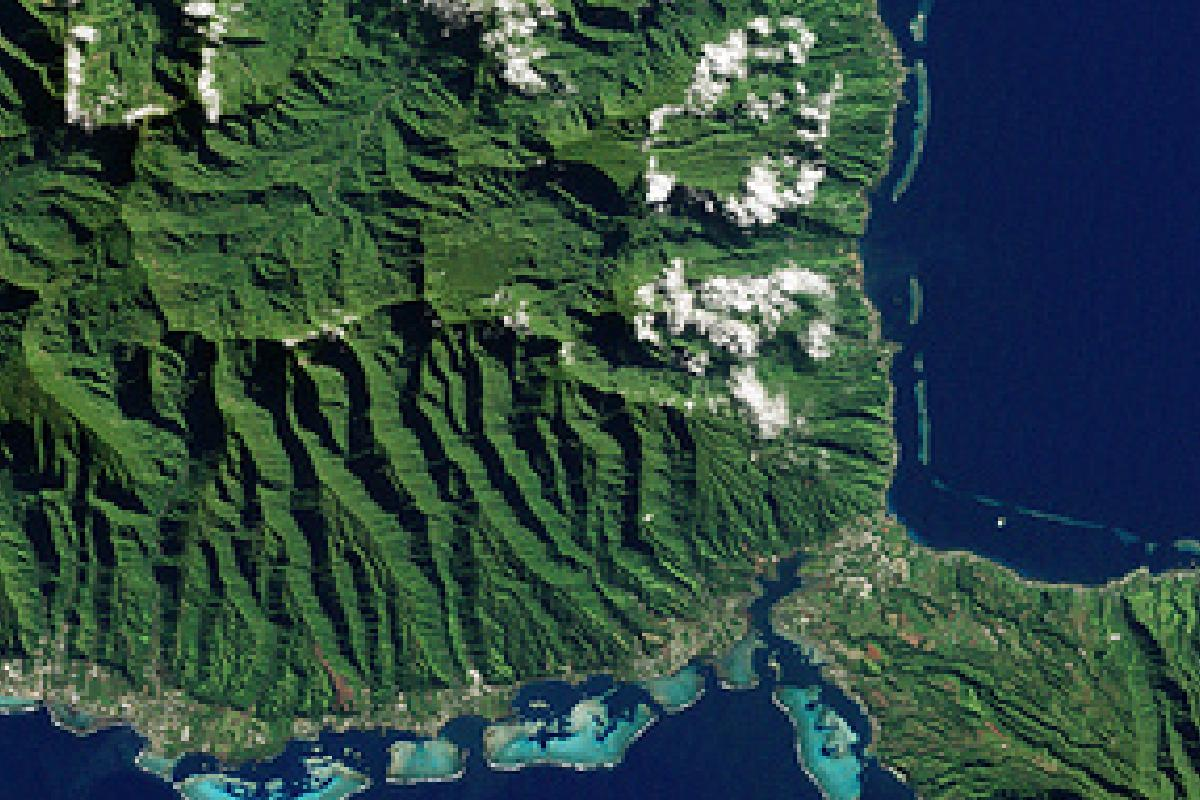
\includegraphics[height=5cm]{screenshot10.jpg}
\caption{Second step of the first test\label{screenshot1Test1}}
\end{figure}

\begin{figure}[htb]
\centering 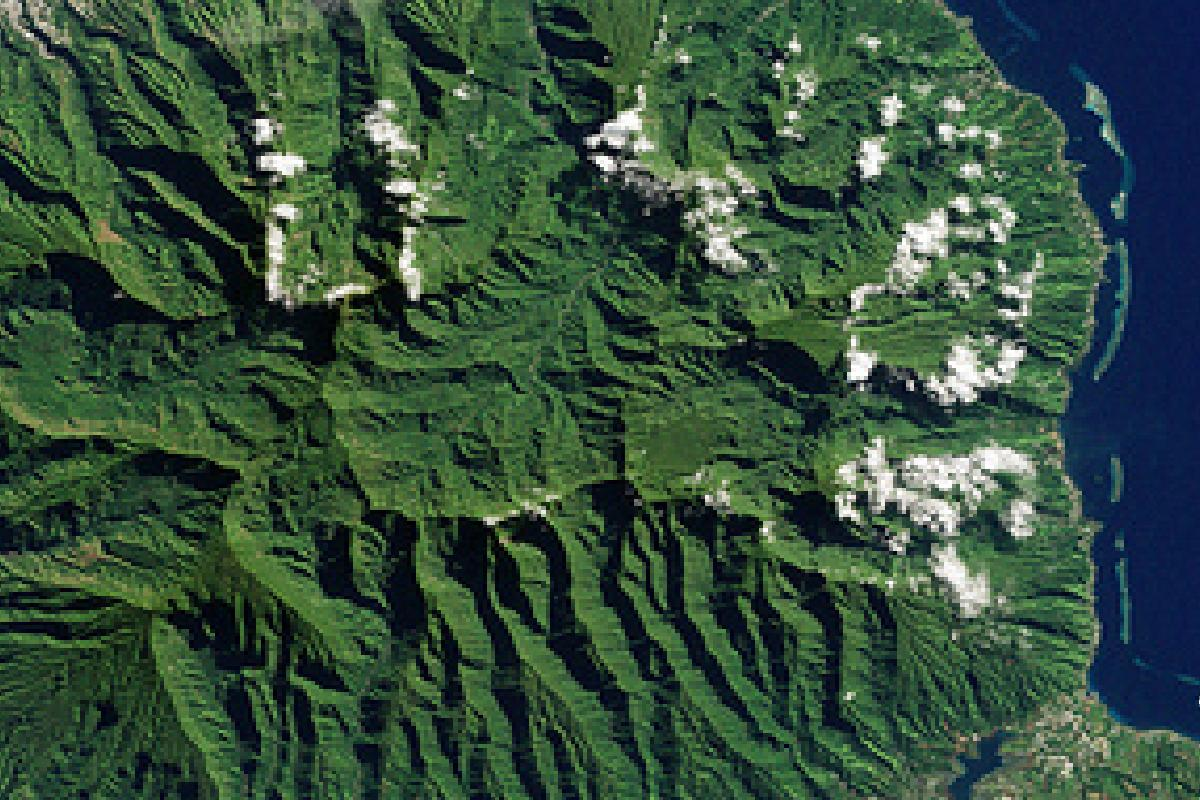
\includegraphics[height=5cm]{screenshot20.jpg}
\caption{Third step of the first test\label{screenshot2Test1}}
\end{figure}

\begin{figure}[htb]
\centering 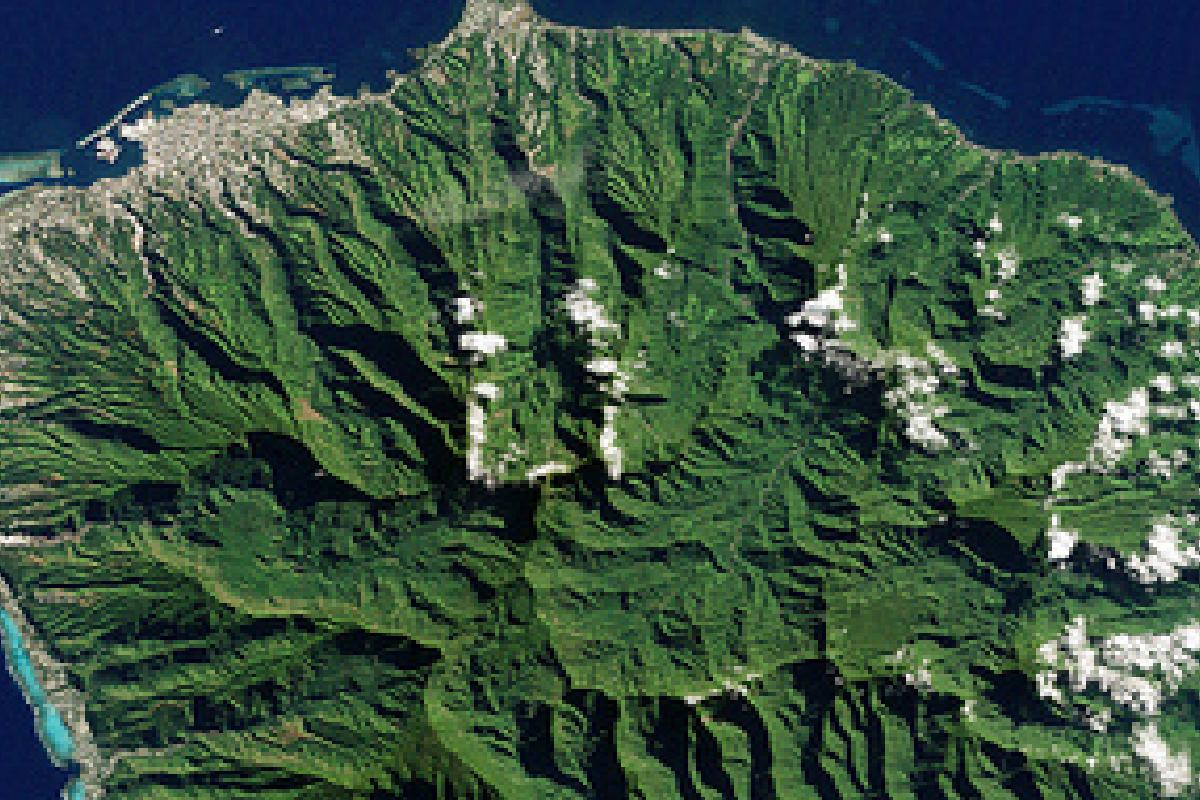
\includegraphics[height=5cm]{screenshot30.jpg}
\caption{Fourth step of the first test\label{screenshot3Test1}}
\end{figure}

\begin{figure}[htb]
\centering 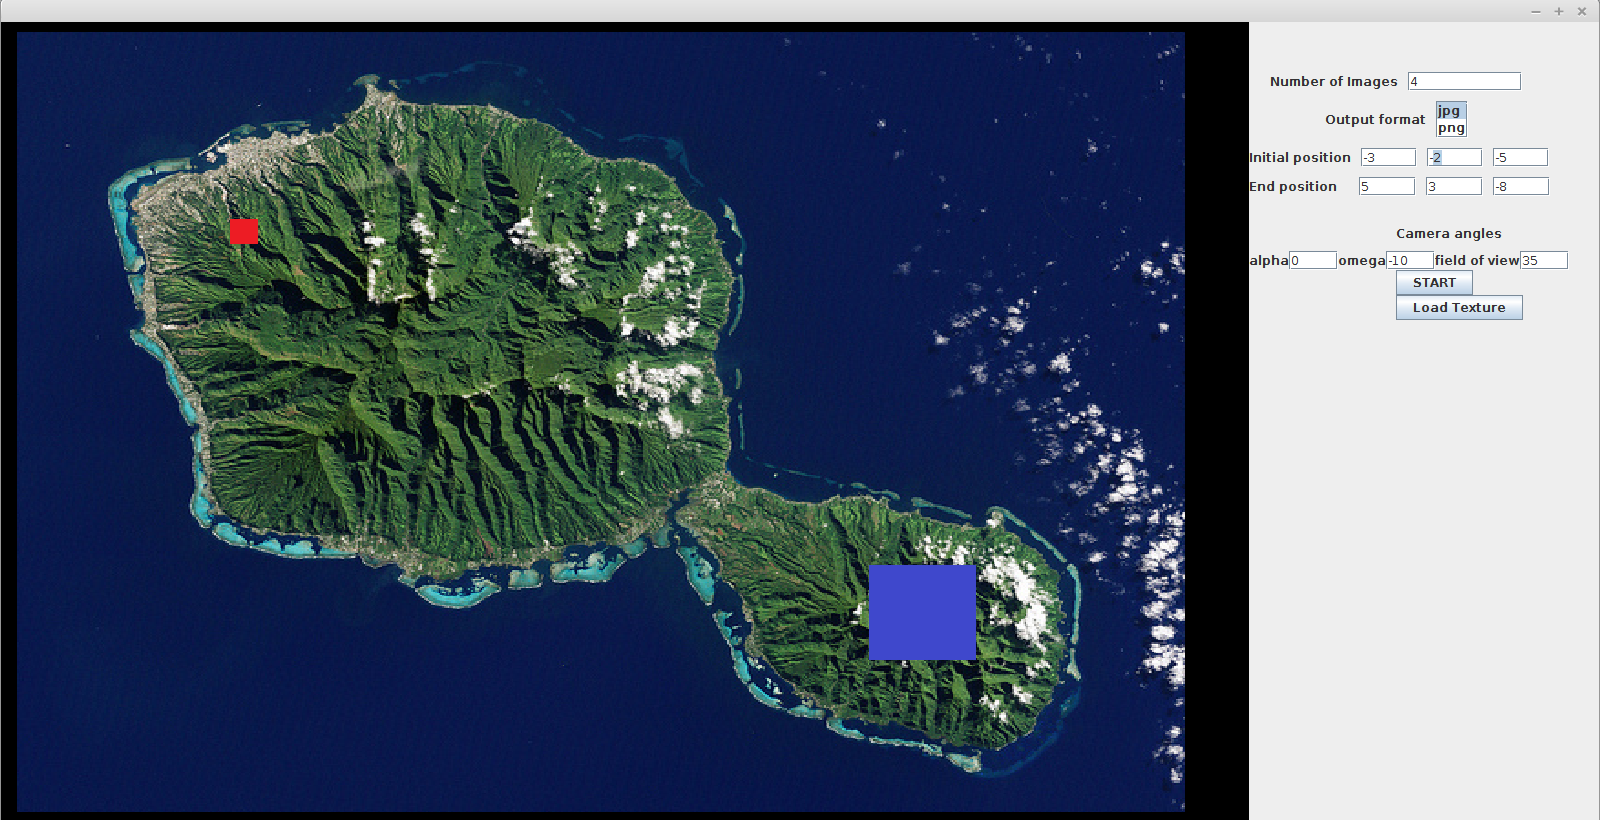
\includegraphics[height=7cm]{screenTest2.png}
\caption{The setup of the second test\label{screenTest2}}
\end{figure}

\begin{figure}[htb]
\centering 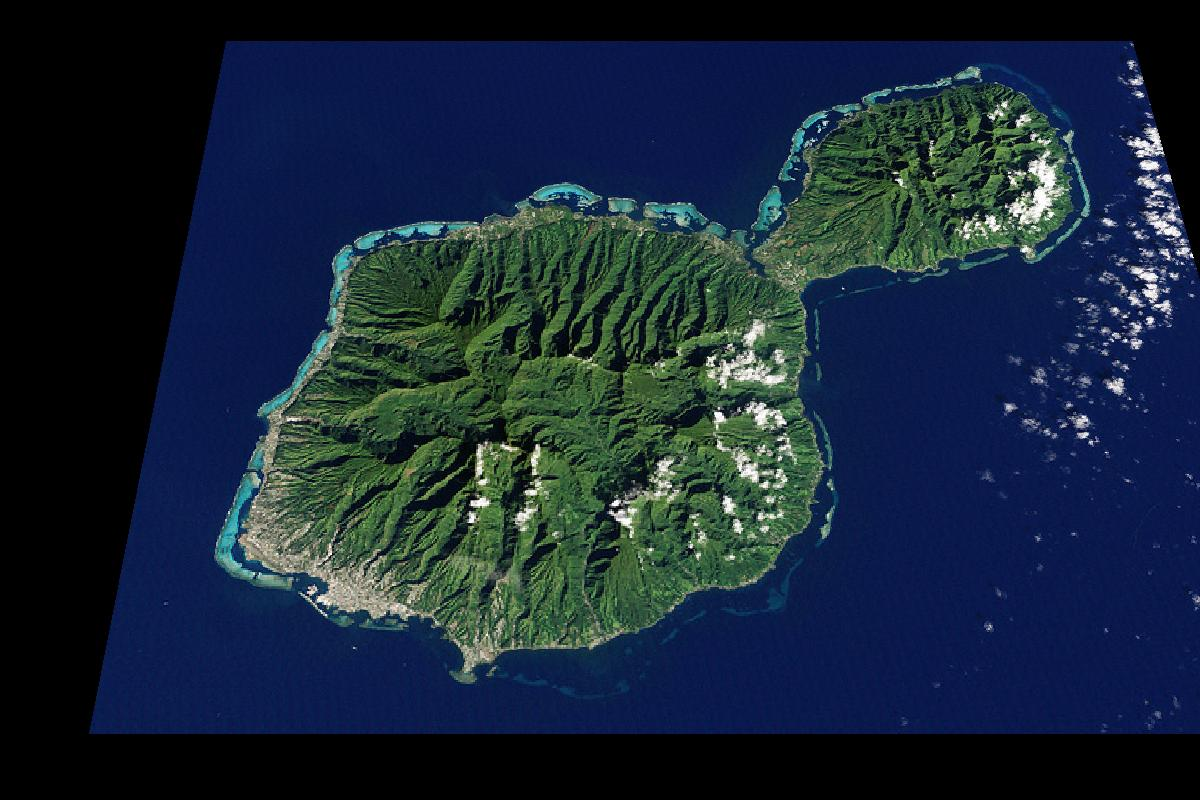
\includegraphics[height=5cm]{screenshot0.jpg}
\caption{First step of the second test\label{screenshot0Test2}}
\end{figure}

\begin{figure}[htb]
\centering 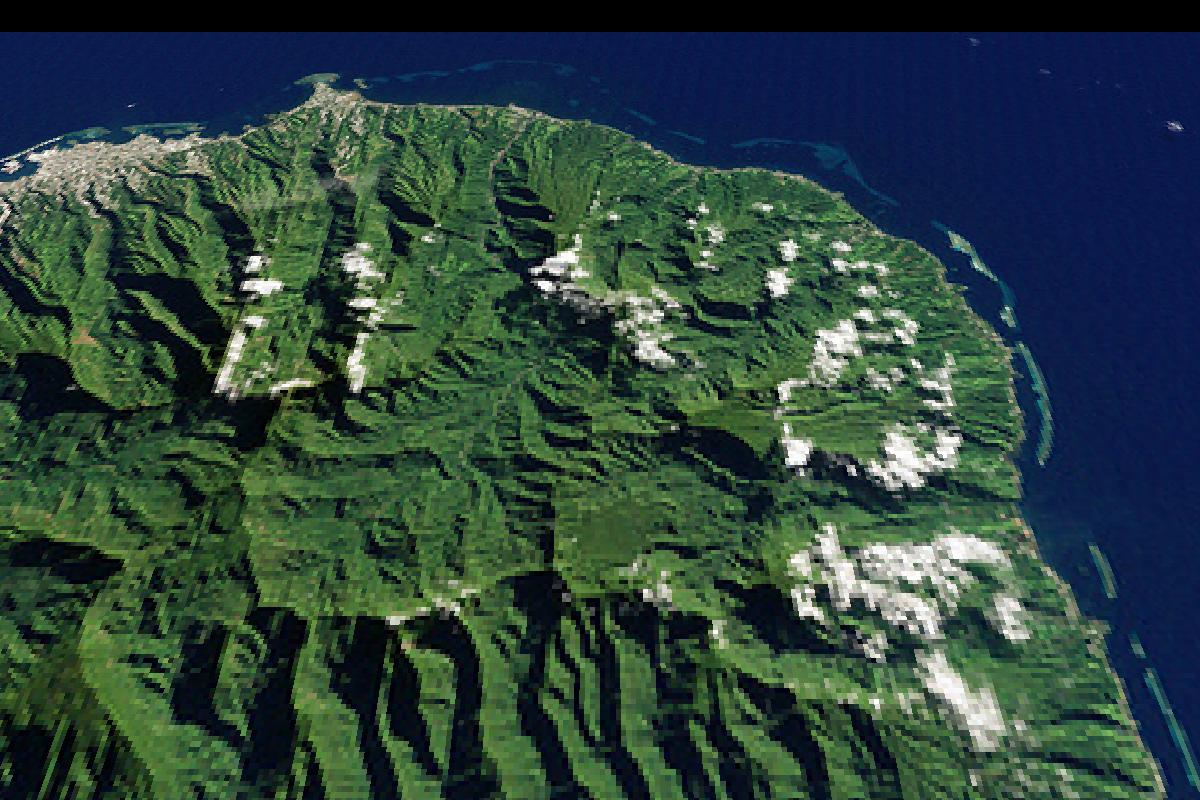
\includegraphics[height=5cm]{screenshot1.jpg}
\caption{Second step of the second test\label{screenshot1Test2}}
\end{figure}

\begin{figure}[htb]
\centering 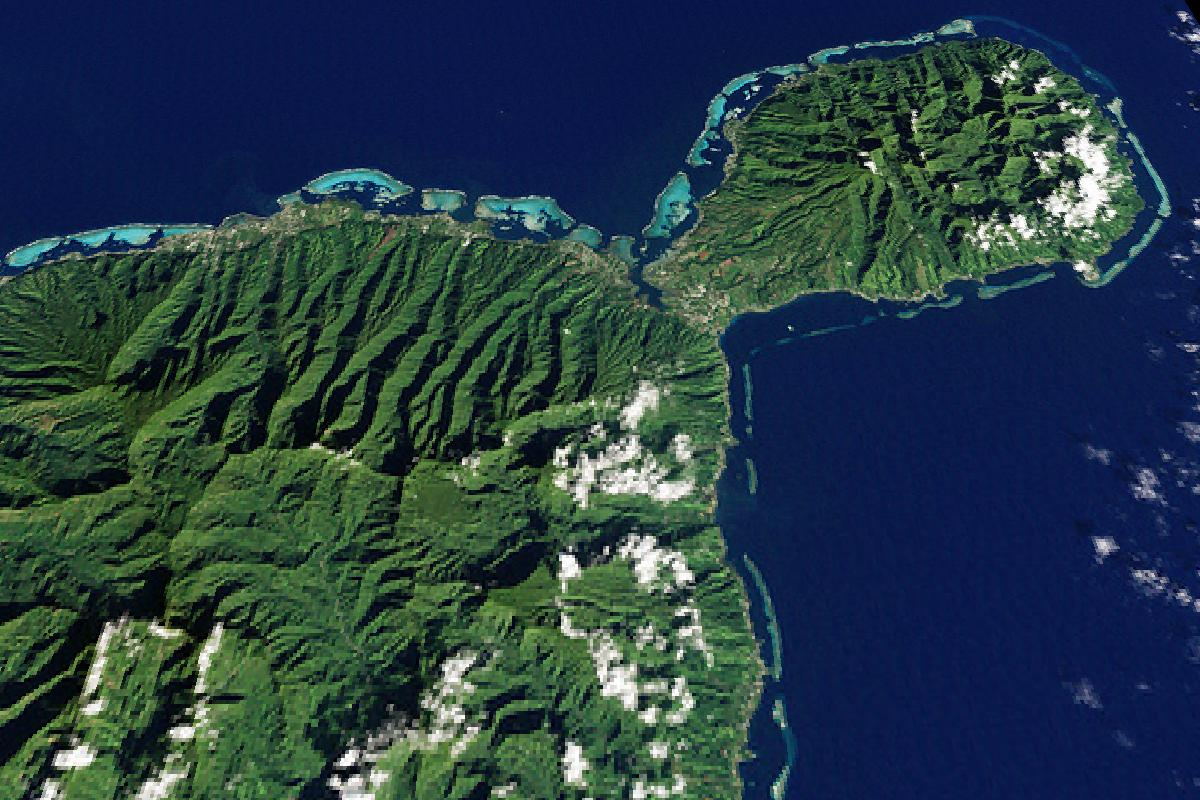
\includegraphics[height=5cm]{screenshot2.jpg}
\caption{Third step of the second test\label{screenshot2Test2}}
\end{figure}

\begin{figure}[htb]
\centering 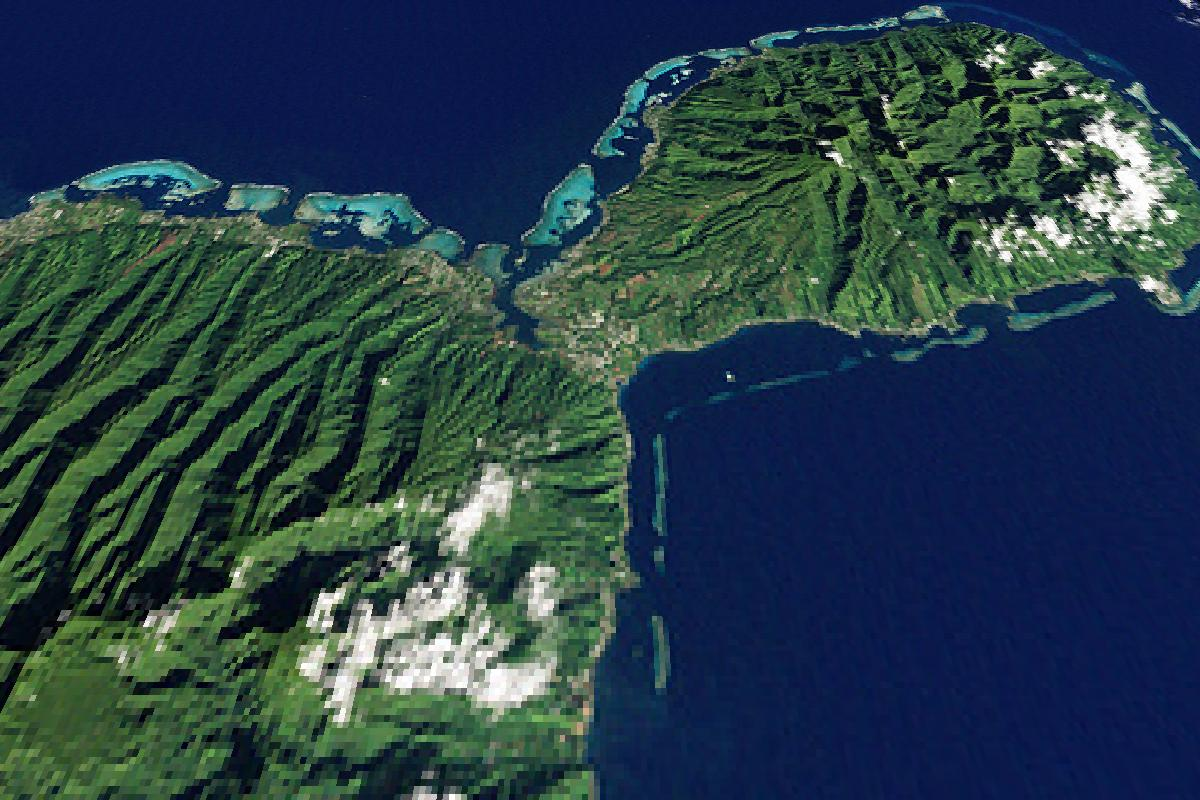
\includegraphics[height=5cm]{screenshot3.jpg}
\caption{Fourth step of the second test\label{screenshot3Test2}}
\end{figure}

\clearpage

\section{Conclusions and future works} 

The aim of this work was to develop an application capable of generating simulated images captured by a camera mounted on a spacecraft during a flight over 2D surface. It can be stated that such application, for simplified setup, was successfully developped and the results are convincing.

Still, there is a lot of room for future development and more improvements. Several suggestions for such improvements are listed below.


\subsection*{Improved GUI and rendering}

The GUI, as stated earlier, is very simple. One of the possible improvements could be switching to another GUI library, for example TWL\cite{TWL} or nifty\cite{Nifty}. That would allow more convenient control, for example adding of sliders for setting the position. Also, the rectangles symbolising the carrier and target are very primitive, therefore a better depiction could be introduced.

Besides those cosmetic changes, also coordinates system could be adjusted. Currently, the span of the x and y coordinates is fixly set from -4.5 to 4.5 for the top view, and the altitude is defined as distance from camera in the range from 0 to 10. For the real world applications, it would be a good idea to add the possibility to specify for example the real size of the 2D plane, and based on this values, the coordinates would be recalculated.

\subsection*{Curved surface}

The primary use of this software is presented as part of the asteroids mission program, but in case it finds its use in another projects, for example concerning Earth imaging, then a nice feature could become a slight curvature of the 2D plane, imitating the curvature of the Earth's surface. 

In order to do so, the 2D plane would have to be changed to 3D sphere. This can be done by using the sphere object from the \textit{lwjgl.util.glu} package \cite{lwjglSphere}. Of course, such sphere would have quite big diameter, compared to the altitude of the spacecraft. 

The problem with rendering of the sphere is the texture mapping. In this work, no sphere textures were used so far, but if it is required in the future, it could be useful to express the coordinates in the spherical coordinate system, or to use the UV mapping technique \cite{UVmappingWiki}. Although, given the error introduced by the curvature is small, it might be possible to just map the texture as if it was 2D plane and accept this error.

\subsection*{Custom 3D surface}

Another extension, similar to the previous one, but more complicated could be loading of arbitrary surface of the 'land'. Such feature could be useful specifically in a project such as the asteroid impact mission, because the surface of the asteriod is very different from 2D plane, and the spacecraft would be close enough to recognize those irregularities.

The first thing such approach needs is a 3D model. The model should be presented in some easily parsable format, such as .obj, because a custom parser has to be created. The loading and parsing of a .obj model is nothing hard and there are tutorials on the internet \cite{Load3DModel}. After the model has been created and loaded into the application, the texture has to be loaded to cover it. This is the hard part, again UV mapping\cite{UVmappingWiki} could be helpful in this case. Unfortunately, 3D texturing is way out of the scope of this work. 

\subsection*{Light intensity and Attenuation}

When simulating images of a surface, it is certainly worth considering the parameters of the light source, it's intensity, position and so on. Also, the parameters of the surface, such as reflexivity could be taken into account. 

The light intensity for every pixel should be calculated in the shader, therefore this is the main class to be modified. There are several ways how to approach this problem, in computer graphics the Lambertian Illumination Model is perhaps the most popular one. The important parameters are: intensity and direction of the incoming light, the distance from the light source, the normal vector, the basic color of the surface and the ambient light intensity.

A nice tutorial about this model and its implementation in java can be found in \cite{ShaderTut}.

This modification would also require change of the GUI, to set the light source parameters.

\subsection*{Curved trajectory}

In this work, only line trajectory of the spacecraft has been assumed. It is sufficient for most of the cases, but a possible improvement could be a curved trajectory, especially in connection with the curved or custom 3D surface. In that case, several other input parameters should be added. Assuming that the shape of the trajectory would be circular, which is the most probable case, such curvature could be specified by adding the coordinates of the center of this hypothetic circle. Using this point and the initial and target point, the trajectory can be calculated, an example is portraited on the figure \ref{CurvedTrajectory}.

\begin{figure}[htb]
\centering 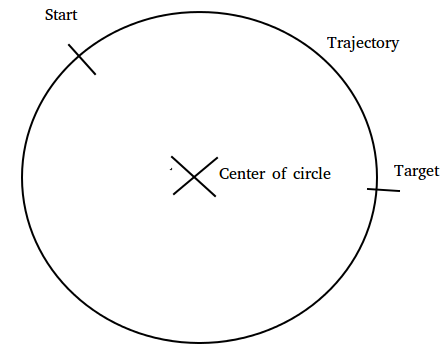
\includegraphics[height=7cm]{CurvedTrajectory.png}
\caption{Curved trajectory scheme\label{CurvedTrajectory}}
\end{figure}

\subsection*{Configuration file and console input} 

In order to automatize the image generation, the configuration file can be created. Then, the parameters can be automatically loaded to the application instead of manually entering them in the GUI.

The configuration file can be a simple text file. An example of such file is in the figure \ref{exampleConfig}.

\begin{figure}[htb]
\centering 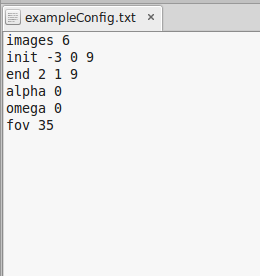
\includegraphics[height=7cm]{exampleConfig.png}
\caption{Example of a configuration file\label{exampleConfig}}
\end{figure}

Such file can be read using the java file parser, reading the file line by line, breaking it into separate strings and then using them as key-value pairs to set up the parameters.

To automatize the process even further, the option of calling the application with parameters from console could be added. The application can be called from console by entering: java -jar CameraProject.jar, parameters can be added at the end of the call and consequently read by the java application, in the \textit{main} method as \textit{args} field. In such manner, the configuration file can be loaded as a parameter.

\clearpage
%% L\"ahdeluettelo
%%
%% \phantomsection varmistaa, ett\"a hyperref-paketti latoo hypertekstilinkit
%% oikein.
%%
%% The \phantomsection command is nessesary for hyperref to jump to the 
%% correct page, in other words it puts a hyper marker on the page.

\phantomsection
\addcontentsline{toc}{section}{\refname}
%\addcontentsline{toc}{section}{References}
\begin{thebibliography}{99}

%% Alla pilkun j\"alkeen on pakotettu oikea v\"ali \<v\"alily\"onti>-merkeill\"a.
\bibitem{AIM} Asteroid impact mission presentation:
	  
$\href{http://www.esa.int/Our_Activities/Space_Engineering_Technology/Asteroid_Impact_Mission}{http://www.esa.int/Our\_Activities/Space\_Engineering\_Technology/Asteroid\_Impact_Mission}$, 5th November, 2016.

\bibitem{ASPECT} ASPECT project presentation:

$\href{http://www.esa.int/Our_Activities/Space_Engineering_Technology/Asteroid_Impact_Mission/ASPECT}{http://www.esa.int/Our\_Activities/Space\_Engineering\_Technology/Asteroid\_Impact\_Mission/ASPECT}$,
  5th November, 2016.

\bibitem{java} Java JDK 1.8 homepage:

    $\href{http://www.oracle.com/technetwork/java/javase/downloads/jdk8-downloads-2133151.html}{http://www.oracle.com/technetwork/java/javase/downloads/jdk8-downloads-2133151.html}$,
  5th November, 2016.

\bibitem{NetBeans} NetBeans homepage:

    $\href{https://netbeans.org/}{https://netbeans.org/}$,
  5th November, 2016.

\bibitem{lwjgl} Lwjgl 2 library page:

    $\href{http://legacy.lwjgl.org/}{http://legacy.lwjgl.org/}$,
  5th November, 2016.

\bibitem{lwjglUtil} Lwjgl util library page:

    $\href{https://github.com/LWJGL/lwjgl/tree/master/src/java/org/lwjgl/util}{https://github.com/LWJGL/lwjgl/tree/master/src/java/org/lwjgl/util}$,
  5th November, 2016.

\bibitem{jinput} Jinput library page:

    $\href{https://github.com/jinput/jinput}{https://github.com/jinput/jinput}$,
  5th November, 2016.

\bibitem{gitHub} The gitHub page of this project:

    $\href{https://github.com/JBurant/Space-Camera}{https://github.com/JBurant/Space-Camera}$,
  5th November, 2016.

\bibitem{eclipse} Eclipse example of setting up lwjgl:

    $\href{http://wiki.lwjgl.org/wiki/Setting_Up_LWJGL_with_Eclipse.html}{http://wiki.lwjgl.org/wiki/Setting\_Up\_LWJGL\_with\_Eclipse.html}$,
  5th November, 2016.

\bibitem{UVmappingWiki} UV mapping page on wikipedia:

    $\href{https://en.wikipedia.org/wiki/UV_mapping}{https://en.wikipedia.org/wiki/UV\_mapping}$,
  5th November, 2016.

\bibitem{TWL} Themable Widget Library (TWL) for java:

    $\href{http://twl.l33tlabs.org/}{http://twl.l33tlabs.org/}$,
  5th November, 2016.

\bibitem{Nifty} Nifty GUI library for java:

    $\href{https://github.com/nifty-gui/nifty-gui/wiki}{https://github.com/nifty-gui/nifty-gui/wiki}$,
  5th November, 2016.

\bibitem{lwjglSphere} Lwjgl sphere javadoc:

    $\href{http://legacy.lwjgl.org/javadoc/org/lwjgl/util/glu/Sphere.html}{http://legacy.lwjgl.org/javadoc/org/lwjgl/util/glu/Sphere.html}$,
  5th November, 2016.

\bibitem{Load3DModel} Video tutorial for loading a 3D model using lwjgl:

    $\href{https://www.youtube.com/watch?v=izKAvSV3qk0}{https://www.youtube.com/watch?v=izKAvSV3qk0}$,
  5th November, 2016.

\bibitem{JarSplice} JarSplice utility homepage:

    $\href{http://ninjacave.com/jarsplice}{http://ninjacave.com/jarsplice}$,
  5th November, 2016.

\bibitem{ShaderTut} Tutorial on light intensity and attenuation:

    $\href{https://github.com/mattdesl/lwjgl-basics/wiki/ShaderLesson6}{https://github.com/mattdesl/lwjgl-basics/wiki/ShaderLesson6}$,
  5th November, 2016.

\end{thebibliography}

%% Appendices
%% Liitteet
\clearpage

\thesisappendix

\section{Installation and usage\label{LiiteA}}

The software project, as well as the source codes and corresponding libraries can be found on Github \cite{gitHub}, from there it can be forked or copied by anyone. 
As stated in section 2, the application has been developped in java programming language (JDK 1.8), using NetBeans IDE. Therefore, in order to run it, installed java is required. Apart from basic java libraries, the libraries: \textit{jinput} \cite{jinput}, \textit{lwjgl} \cite{lwjgl} and \textit{lwjgl util} \cite{lwjglUtil} have been used. It can be run on any standard operation system (e.g. Windows, LinuxMint, Ubuntu etc.) Although, the native file is specific, therefore, it needs to be build separately for different operating systems, with different value of the native path.

The hardware requirements are not strict, any standard computer with installed java and decent graphics card is suitable. During testing, there was an issue with performance, using a notebook with just integrated graphics card, therefore a PC with standard graphics card is recommended. 

The library lwjgl (lightweight java openGL library) enables to use the openGL in the java application, providing interface to the lower level C++ openGL methods. The usage of this library is straightforward, and is very similar to using normal openGL in C++. There are also many tutorials on the internet, providing guidance for the development. An important thing to notice is that the application is using lwjgl2. There is already newer version, lwjgl3, whose interface is slightly different and should not be mixed with version 2. The older version has been chosen, because the newer one didn't provide support for any GUI libraries at the time of development of this application.

The Github bundle contains also prepared NetBeans project, which has those libraries already imported. Only thing that must be changed in the project specification is the java path to the native libraries. To do that, right click on libraries in the project tab and select properties, in the newly opened window, in the categories select Run and specify VM Options as :-Djava.library.path="Path-to-lwjgl-library/lwjgl-2.9.3/native/Desired-OS" (\ref{setUpPaths}).

\begin{figure}[htb]
\centering 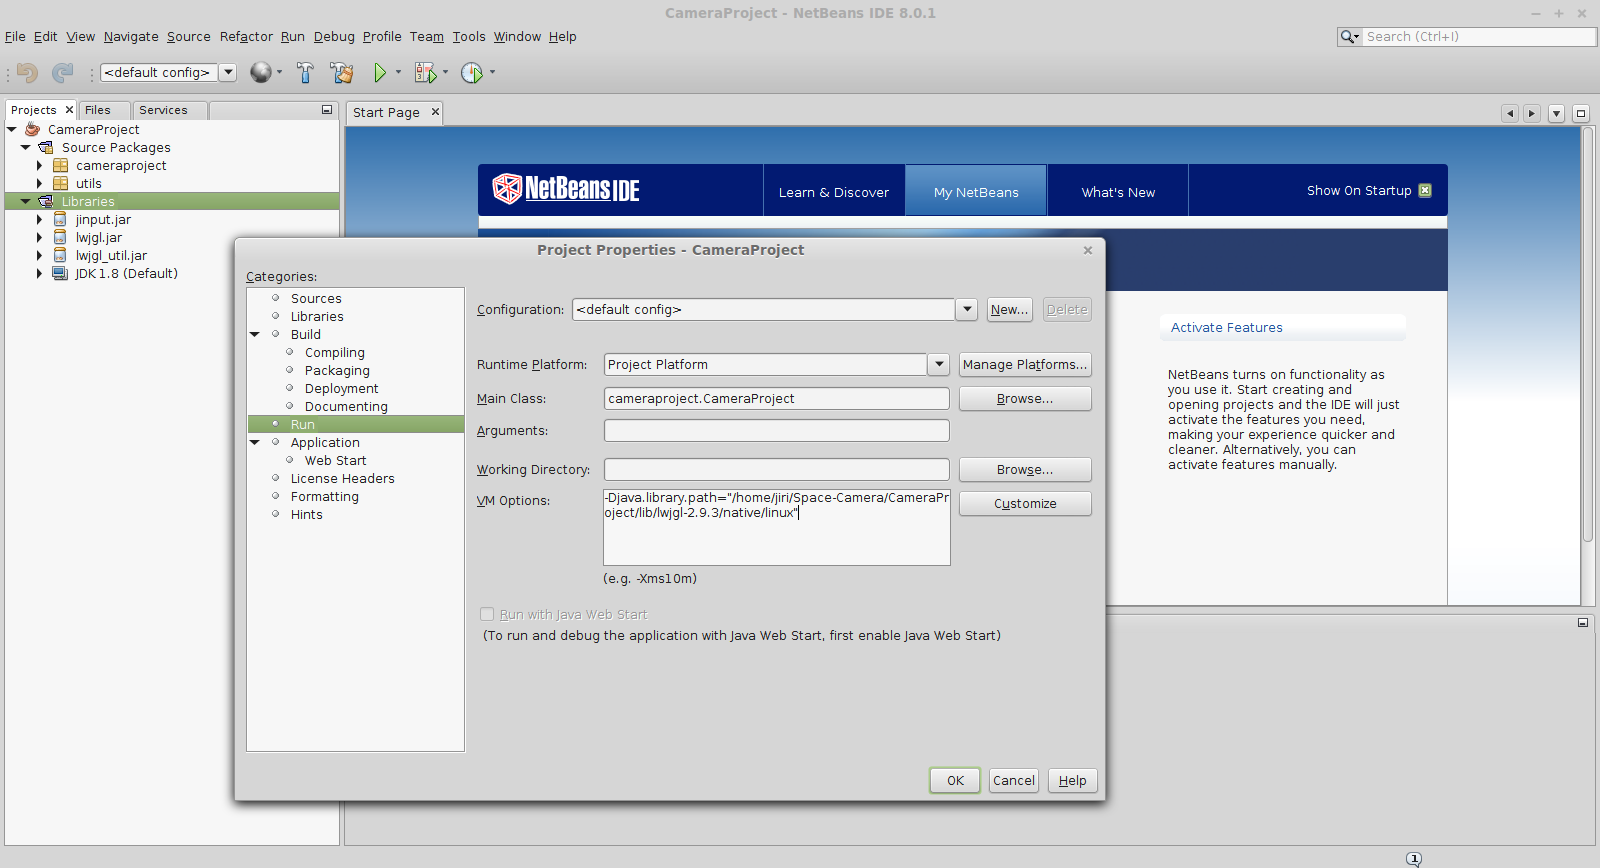
\includegraphics[height=7cm]{SetUpPaths.png}
\caption{Setting up native path in NetBeans IDE\label{setUpPaths}}
\end{figure}

In case, that future development will be carried on using another IDE, the libraries must be added, and the path to native libraries must be set. An example of how to do that in eclipse can be found in \cite{eclipse}.

After the initial imports and after setting the path, no more setup should be needed. 

The application can be compiled using the IDE and consequently run.
It can also be run as already compiled .jar file. 

In order to compile and deploy a new .jar file, a so called fat jar must be created. This can be done for example using the  JarSplice tool \cite{JarSplice}, which packs the project libraries as well as corresponding native libraries into one executable jar folder.

Step-by-step creation of such "fat jar" is shown in the figures below.

In this case only java needs to be installed. Then it can be run for example from the console by typing: "java -jar CameraProjectFat.jar" As for the output of the program, the images are automatically stored to a folder with relative path "./img/screenshots", therefore such folder must exist beforehand.

\begin{figure}[htb]
\centering 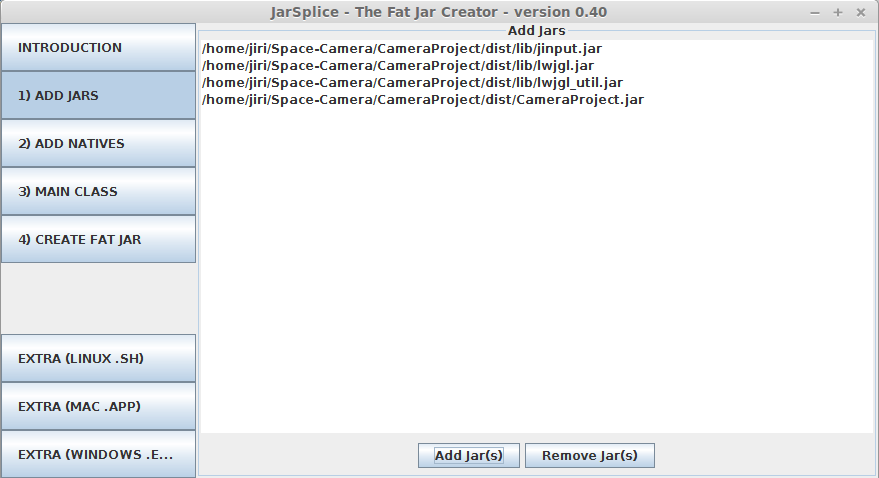
\includegraphics[height=7cm]{jarSplice1.png}
\caption{Building fat jar: Step1\label{jarSplice1}}
\end{figure}

\begin{figure}[htb]
\centering 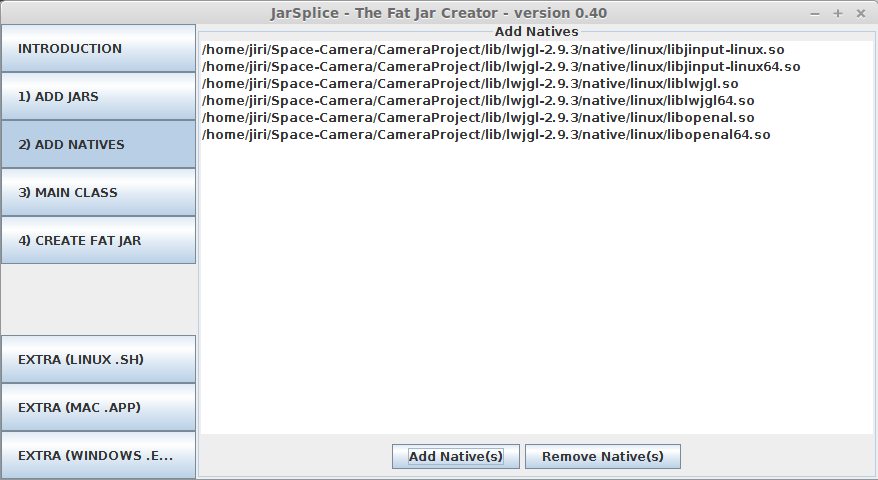
\includegraphics[height=7cm]{jarSplice2.png}
\caption{Building fat jar: Step2\label{jarSplice2}}
\end{figure}

\begin{figure}[htb]
\centering 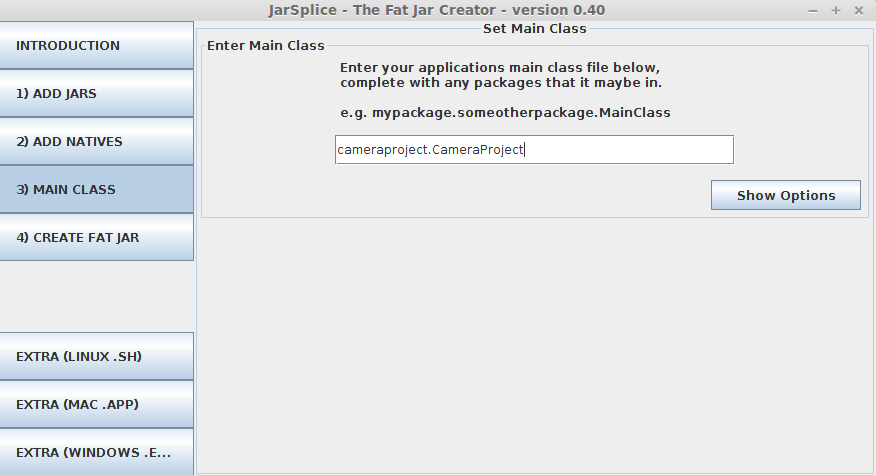
\includegraphics[height=7cm]{jarSplice3.png}
\caption{Building fat jar: Step3\label{jarSplice3}}
\end{figure}

\begin{figure}[htb]
\centering 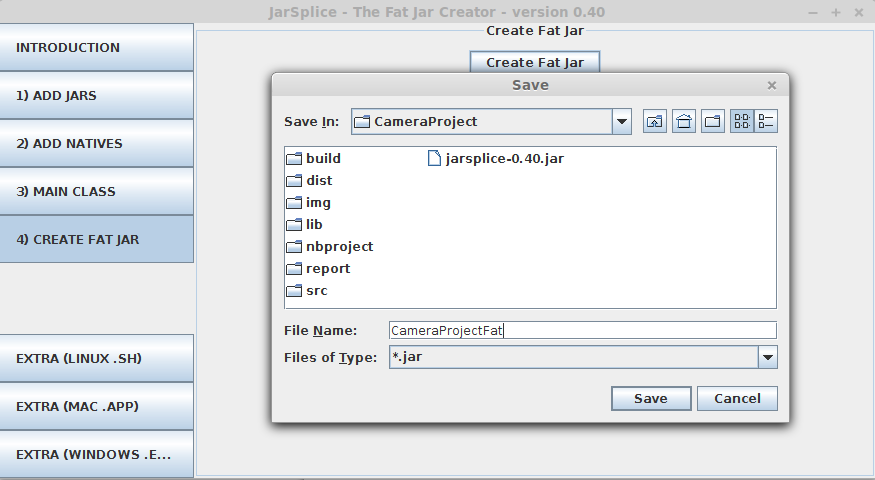
\includegraphics[height=7cm]{jarSplice4.png}
\caption{Building fat jar: Step4\label{jarSplice4}}
\end{figure}

\begin{figure}[htb]
\centering 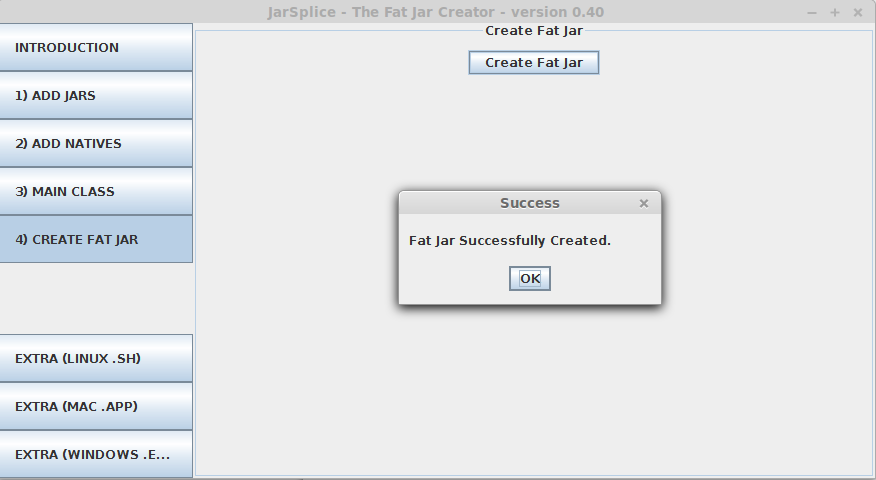
\includegraphics[height=7cm]{jarSplice5.png}
\caption{Building fat jar: Step5\label{jarSplice5}}
\end{figure}

\end{document}
